\section{BİLGİSAYAR AĞLARI MODELLEME}
Bu başlıkta simülatör ve emülatör kavramları açıklanmaya çalışılıp örnek uygulamalar verilecektir.

\subsection{Simülatör \& Emülatör}

Bilgisayar üzerinde bir ağı modellemek için; simülatör ve emülatör şeklinde iki tür program kullanılmaktadır:

\textbf{Simülatör}: Gerçek ortamdaki sistemler ile (çok benzese de) birebir aynı şekilde çalışmaz. Uçuş simülatörleri buna örnek gösterilebilir. Gerçek sistemlerde kullanılan donanımların üzerindeki yazılımlar bunda kullanılmaz, simülatörlerde kullanılan sanal cihazlarda özel geliştirilmiş ve kısıtlı yazılımlar çalışır. Ayrık zamanda çalışır: gerçek hayatta binlerce saat sürecek bir işlem 1 saniyede yapılabilir;  gerçek hayatta 1ms içerisinde biten bir eylem saniyelerce sürecek şekilde yavaşlatılabilir.

\vskip 0.5cm
\textbf{Emülatör}: Gerçek cihazlarda kullanılan yazılımlar doğrudan burada da çalıştırılır. Virtualbox üzerinde Windows çalıştırmak için, gerçek Windows kurulumu yaptığımızı hatırlayın. Donanımlar sanallaştırılır ama donanımlar üzerinde gerçek yazılımlar (işletim sistemleri) kullanılır. Gerçek zamanda çalışır.

\vskip 0.5cm
Simülatör ve emülatör kavramlarını bilgisayar ağları konusu özelinde özetlemeye çalışalım.
\vskip 0.5cm

İnternet'in ortak dilinin IP olması gibi, bilgisayar ağlarında ortak donanım da Cisco firmasının ürünleridir. Pazara erken girmiş olması, ürünlerinin kaliteli olması, geniş ürün yelpazesi olması, bol miktarda dokümanı olması, kullanıcı sayısının çok olması, vb. nedenlerle bilgisayar ağları çalışan hemen herkes Cisco cihazlara hakim olmaktadır. Bu nedenle, ağ modelleme programlarında öncelikle Cisco cihazlara (yönlendirici, anahtar, vb.) destek sağlanmaktadır.

Emülatör uygulamalarında, \textit{-simülatörlerden farklı olarak-} gerçek Cisco işletim sistemi kullanılması gerekmektedir. Gerçek işletim sistemi kullanıldığı için, gerçek cihazlarla yapılan fiziksel ağ uygulamalarına çok yakın bir çalışma ortamı sağlamaktadır. Bunun en büyük dezavantajı ise Cisco işletim sistemleri ücretli olduğu için ilave maliyet çıkarmasıdır. Diğer taraftan; bu işletim sistemlerinin İnternet'in yeraltı dünyasında yaygınlaşması gibi illegal durumlara da sebebiyet vermektedir.

\subsection{Ağ Modelleme Platformları (Ücretsiz Olanlar)}
\subsubsection{Cisco Packet Tracer}
Cisco firması tarafından geliştirilmektedir. Cisco'nun Networking Academy adı altında vermiş olduğu eğitimlerde katılımcılara verilmektedir. Bunun haricinde satışı bulunmamaktadır. Simülatör tarzında bir uygulamadır.

\begin{figure}[H]
    \centering
    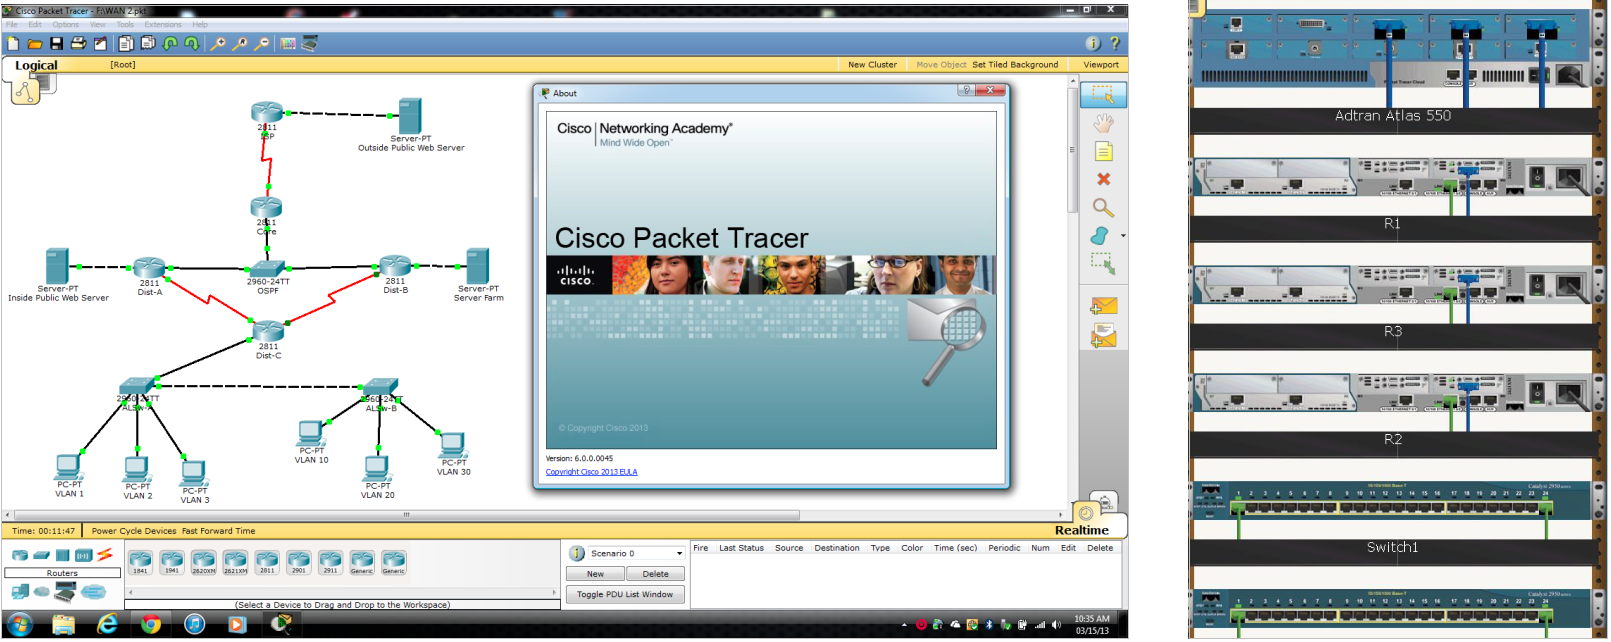
\includegraphics[width=\textwidth]{images/SimulatorCiscoPT.png}
    \caption{Cisco Packet Tracer arayüzü. Sol tarafta "mantıksal", sağ tarafta "fiziksel" görünüm}
    \label{fig:CiscoPT}
\end{figure}

Kataloğunda Sadece Cisco firmasına ait ürünler bulunmaktadır. Yönlendirici, anahtar, kablosuz erişim noktası, IP telefon sistemler, vb. farklı türde ürünler kullanılabilmektedir. Linux ve Windows sürümleri bulunmaktadır. Program kurulduğunda, ilave bir işlem yapmaya gerek kalmadan tüm özellikleri ile aktif halde olmaktadır. Program içerisinde oluşturulan sanal cihazların gerçek hayat ile bağlantısı yapılamamaktadır. Sadece klasik bilgisayar ağları değil, üst katmanlarda da uygulama gerçekleştirilebilmektedir. Sanal sunucu cihazı üzerinden HTTP, DNS, e-posta sunucuları gibi servisler de simüle edilebilmektedir.

\subsubsection{GNS3 (Graphical Network Simulator 3)}
Cisco'nun kendi cihazları için tasarladığı IOS isimli işletim sistemlerini kullanır. Bu IOS'lerden GNS3 içerisine en az 1 tane dahil edilmelidir. Bu IOS'leri elde etmek için yasal bir yol malesef bulunmamaktadır. Cisco müşterisi olanlar WEB üzerinden indirebilmektedir. Bunun haricinde satışı bulunmamaktadır. VirtualBox PC'leri bunun içine dahil edilebilmektedir. Gerçek yönlendirici imajları ve gerçek sanal bilgisayarlar kullandığından oldukça gerçekçi bir çalışma ortamı sağlamaktadır. Cisco sertifikasyon sınavlarına hazırlananlar için de kullanışlıdır. Programın önemli bir özelliği de sanal ağda kullanılan sanal makinaların Host-PC (fiziksel bilgisayar) üzerinden internet'e çıkabilmesidir.

\begin{figure}[H]
    \centering
    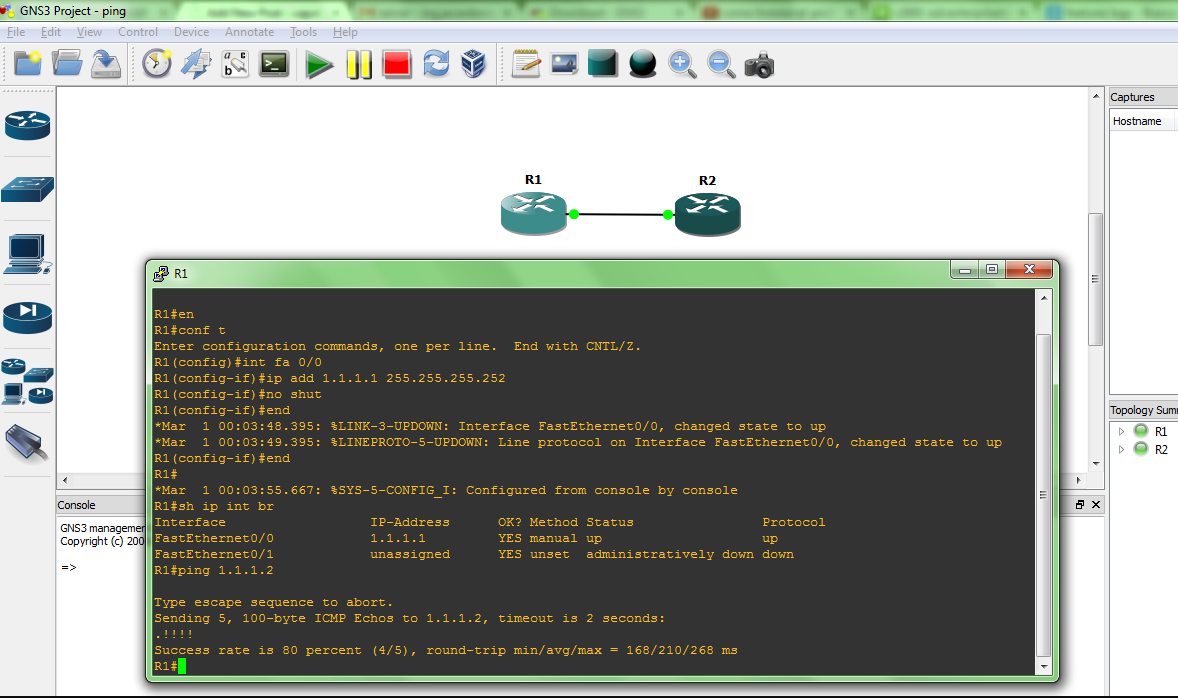
\includegraphics[width=\textwidth]{images/SimulatorGNS3.png}
    \caption{GNS3 arayüzü içindeki yönlendiricinin konsolu}
    \label{fig:GNS3}
\end{figure}

\subsubsection{CORE (Common Open Resource Emulator) }
Linux ve BSD üzerinde çalışıyor. Windows üzerinde sanal bilgisayarda çalıştırılabiliyor. Hatta kendi sitesinde, VmWare Player için hazır imajları da var. CORE içindeki her bir sanal PC'de Linux çalışıyor. Sanal ağ üzerinde lazım olan tüm işlevleri bu Linux'lar vasıtasıyla gerçekleştirilebiliyor. DHCP sunucusu, yönlendirici hizmeti, WEB sunucusu, vb. tüm işlevler Linux platformları üzerinden sağlanabiliyor. Yönlendirici olarak Cisco kullanma alışkanlığı olanlar, bir sanal Linux üzerine Quagga kurarak, onu sahte Cisco yönlendiriciye çevirebilirler.

Sanal ağı, gerçek ağa bağlayarak internet'e çıkarma özelliği bulunmaktadır. Büyük projelerde kullanmak üzere dağıtık hesaplama desteği de bulunmaktadır. Örneğin; elinizde 3 tane fiziksel PC varsa ve 200 tane node'dan oluşan sanal bir ağ kullanmak istiyorsanız, node'ları iki fiziksel PC'ye paylaştırabilir, 1 PC'yi de GUI amacı ile kullanabilirsiniz. Phyton ile script yazılabildiğini de belirtelim.

\begin{figure}[H]
    \centering
    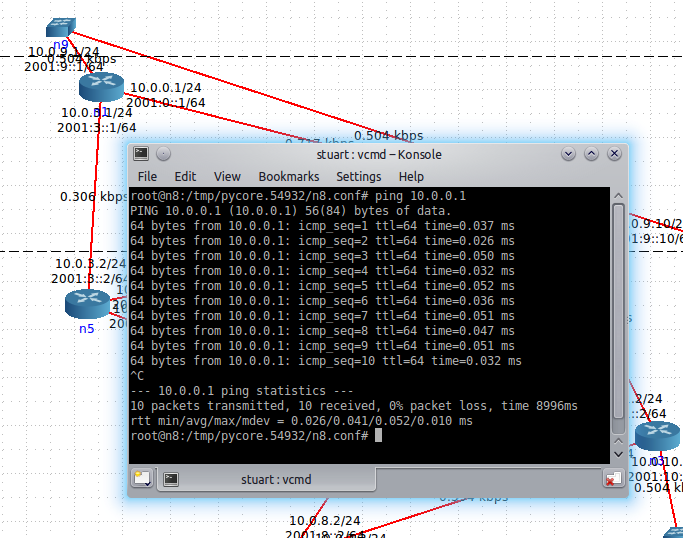
\includegraphics[width=\textwidth]{images/SimulatorCORE.png}
    \caption{CORE ekran görüntüsü}
    \label{fig:CORE}
\end{figure}

\subsubsection{Diğerleri}

\begin{itemize}
\item \textbf{NS2:} \url{http://www.isi.edu/nsnam/ns/}
\item \textbf{NS3:} \url{https://www.nsnam.org/} (NS2'nin devamı olarak yapılmasına rağmen geriye doğru uyumluluğu
olmadığından ayrı bir yazılım olarak değerlendiriliyor)
\end{itemize}

\begin{itemize}
\item \textbf{Cloonix}: \href{http://clownix.net/}{http://clownix.net} Açık kaynaklı. KVM sanal makine desteği var.
\item \textbf{IMUNES}: \href{http://www.imunes.net/}{http://www.imunes.net} Açık kaynaklı. FreeBSD üzerinde çalışıyor.
Sanal makinede çalıştırılabilir.
\item \textbf{OMNeT++}: \url{http://www.omnetpp.org/}
\item \textbf{Marionnet}: \url{http://www.marionnet.org/EN/}
\item \textbf{Mininet}: \href{http://www.mininet.org/}{http://www.mininet.org}
\item \textbf{Netkit:} \href{http://wiki.netkit.org/}{http://wiki.netkit.org}
\item \textbf{Psimulator2:} \url{http://code.google.com/p/psimulator/}
\item \textbf{Virtualsquare:} \url{http://wiki.virtualsquare.org/wiki/index.php/Main_Page}
\item \textbf{VNX and VNUML:} \url{http://www.dit.upm.es/vnx}
\item \textbf{OPNET (Ücretli):} \url{http://www.riverbed.com/products/performance-management-control/opnet.html}
\end{itemize}
\section{Kaynaklar}

\begin{enumerate}
\item \url{http://www.brianlinkletter.com/open-source-network-simulators/}
\item \url{http://www.finmars.co.uk/blog/4-evaluating-network-simulation-tools}
\item \url{http://nil.uniza.sk/network-simulation-and-modelling/network-simulators-list}

\bigskip
\end{enumerate}